\documentclass[10pt]{article}

% The following command leaves more space between lines.  That's great
% when correcting drafts.  When you comment it out, however, the
% output looks much nicer.
%
\linespread{1.0}

\usepackage{amsmath}
\usepackage{amssymb}
\usepackage{graphicx}
\usepackage{epsfig}
\usepackage{latexsym}
\usepackage{amsthm}

\usepackage{mathrsfs}

\usepackage{multicol}



\usepackage[colorlinks,citecolor=blue]{hyperref}

\usepackage[latin1]{inputenc}

\usepackage{tikz-cd}
\usepackage{pgfplots}

%\usepackage{3dplot}

\usetikzlibrary{matrix,arrows,decorations.pathmorphing}


\usepackage[scale=0.8]{geometry}


%\usepackage{umoline}\setlength{\UnderlineDepth}{1pt}
%\usepackage[linktocpage=true]{hyperref}

\input xy
\xyoption{all}


%\addtolength{\hoffset}{-.5in}
%\addtolength{\textwidth}{1in}
%\setlength{\parindent}{.5in}
%\setlength{\textheight}{9.5in} \setlength{\topmargin}{-2cm}


\pagestyle{myheadings}\parindent 0em




\usepackage[latin1]{inputenc}


%------------------copy and posted code from the internets-------------

%\numberwithin{equation}{section} % comment out when neccessary

\newtheorem{theorem}[equation]{Theorem}
\newtheorem{lemma}[equation]{Lemma}
\newtheorem{proposition}[equation]{Proposition}
\newtheorem{corollary}[equation]{Corollary}


\theoremstyle{definition}
\newtheorem{definition}[equation]{Definition}
\newtheorem{example}[equation]{Example}
\newtheorem{remark}[equation]{Remark}
\newtheorem{problem}[equation]{Problem}



\newcommand{\R}[1]{\mathbb{R}^{#1}}
\newcommand{\C}[1]{\mathbb{C}^{#1}}
\newcommand{\Z}[1]{\mathbb{Z}^{#1}}
\newcommand{\K}[1]{\mathbb{K}^{#1}}
\newcommand{\embed}[0]{\hookrightarrow}
\newcommand{\TT}[4]{\begin{tabular}{| c | c |}\hline $#1$ & $#2$ \\ \hline $#3$ & $#4$ \\ \hline\end{tabular}} %goddamn it
\newcommand{\partd}[2]{\frac{\partial #1}{\partial #2}}
\newcommand{\limit}[2]{\displaystyle{ \lim_{#1 \to #2}}}
\newcommand{\vectornorm}[1]{\left|\left|#1\right|\right|}
\newcommand{\Ker}[0]{\text{\textnormal{Ker}}}
\newcommand{\Hom}[0]{\text{\textnormal{Hom}}}
\newcommand{\circled}[1]{\tikz[baseline=(char.base)]{
            \node[shape=circle,draw,inner sep=2pt] (char) {#1};}}


\newcommand{\T}{\rotatebox[origin=c]{180}{$\scriptscriptstyle \perp $}}
\newcommand{\x}{\textbf{x}}
\newcommand{\y}{\textbf{y}}
\newcommand{\supp}{\text{\textnormal{supp}}}
\newcommand{\csupp}{\text{\textnormal{cosupp}}}
\newcommand{\found}{\text{\textnormal{found}}}
\newcommand{\roof}{\text{\textnormal{roof}}}

\newcommand{\bcup}{\displaystyle\bigcup}
\newcommand{\bcap}{\displaystyle\bigcap}
\newcommand{\dsum}{\displaystyle\sum}
\newcommand{\dint}{\displaystyle\int}





\begin{document}
%

{\bf Name:} \hrulefill\hrulefill\hrulefill\\
{\bf M143} \qquad \qquad \\
{\bf Polynomials}\\ %(look familiar??)\\
%Show all work for full/partial credit.
%---------------- End of the document ---------------
\begin{definition}
A \textit{polynomial} $p(x)$ is a function that can be written in the form $$p(x)=a_nx^n+a_{n-1}x^{n-1}+\cdots+a_1x^1+a_0(x^0),$$ where $n\geq 0$ is a whole number, and $a_n\neq 0$ \textbf{unless} $p(x)=0$.

\begin{itemize}
\item The $a_i$ are the \textit{coefficients} of $p(x)$.
\item $a_n$ is the \textit{leading coefficient} of $p(x)$.
\item $n$ is the \textit{degree} of $p(x)$.
\item $a_nx^n$ is the \textit{leading term}  of $p(x)$.
\end{itemize}


\end{definition}

\section{Long Term Behavior}

When we consider a polynomial $p(x)=a_nx^n+a_{n-1}x^{n-1}+\cdots+a_1x^1+a_0$, we notice that no matter how big the coefficients $a_{n-1}$ through $a_0$ are, they will all eventually be made insignificant by $x^n$ for some sufficiently large values of $x$.  Thus we have the following fact:

\begin{remark}
The long term behavior of $p(x)$ is determined \textbf{completely} by it's leading term $a_nx^n$.
\end{remark}

So we have 2 things to consider, whether or not $a_n$ is positive or negative, or whether or not $n$ is even or odd. \\

If $a_n>0$, then there are 2 possibilities:

\begin{itemize}
\item If $n$ is even, (like $x^2, x^4, x^6)$, then $a_nx^n$ cannot be negative, so $p(x)$ will tend to positive infinity as $x$ goes to either positive or negative infinity.
\item If $n$ is odd, (like $x, x^3, x^5)$, then $a_nx^n$ is positive as long as $x$ is positive, so $p(x)$ will tend to positive infinity as $x$ goes to either positive infinity, and $a_nx^n$ will go to negative infinity as x goes to negative infinity.
\end{itemize}
Then, if $a_n<0$, everything is flipped upside down.  We can summarize as follows:
$$
\begin{tabular}{c|c|c|}
 & $n$ even & $n$ odd\\
\hline 
$a_n>0$ & $p(x)\to \infty$ as $x\to \infty, -\infty$& $p(x)\to  \begin{cases}\infty & x\to \infty\\ -\infty & x\to -\infty \end{cases}$\\
\hline 
$a_n>0$ & $p(x)\to -\infty$ as $x\to \infty, -\infty$& $p(x)\to  \begin{cases}-\infty & x\to \infty\\ \infty & x\to -\infty \end{cases}$\\
\hline
\end{tabular}
$$
\section{Short Term Behavior}
The first thing one can always do when analyzing the short term behavior of $p(x)$ is find the $y$-intercept.  The $y$ intercept is just the point on the curve of the function when $x=0$, so this is $p(0)=a_0$.\\

By the \textbf{Fundamental Theorem of Algebra}, we can write $p(x)=a_nx^n+\cdots +a_0$ as: $$p(x)=a_n(x-r_1)^{m_1}(x-r_2)^{m_2}\cdots (x-r_k)^{m_k}\cdot q_1(x)q_2(x)\cdots q_\ell(x)$$
where the $q_i(x)$ are irreducible quadratics.  We call $r_1, \ldots, r_k$ the \textit{roots} of $r(x)$, where root $r_i$ has \textit{multiplicty} $m_i$.  What this means is if we plug $r_i$ into $p(x)$, we end up with 0, since that linear factor ends up being 0.\\

The behavior of $p(x)$ around these roots is determined by the multiplicity of that root.  We know that $p(x)$ will be 0 at those roots, so the question is whether or not the polynomial crosses the $x$ axis at a given roots, or bounces off the axis:

$$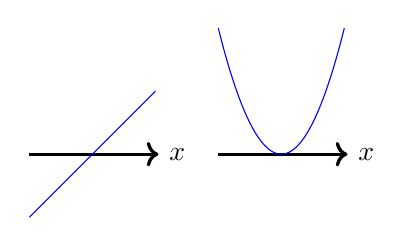
\begin{tikzpicture}[scale=.4][domain=-2:2]
%    \draw[gray!50, thin, step=1] (-10,-5) grid (11,5);
    \draw[very thick,->] (-2,0) -- (2.1,0) node[right] {$x$};
%    \draw[very thick,->] (0,-5) -- (0,5.1) node[above] {$y$};

%    \foreach \x in {-10,...,10} \draw (\x,0.05) -- (\x,-0.05) node[below] {\tiny\x};
%    \foreach \y in {-4,...,4} \draw (-0.05,\y) -- (0.05,\y) node[right] {\tiny\y};


  \draw[scale=1,domain=-2:2,smooth,variable=\x,blue] plot ({\x},{\x});% node[above]{$f(x)$};

    \draw[very thick,->] (4,0) -- (8.1,0) node[right] {$x$};
%    \draw[very thick,->] (0,-5) -- (0,5.1) node[above] {$y$};

%    \foreach \x in {-10,...,10} \draw (\x,0.05) -- (\x,-0.05) node[below] {\tiny\x};
%    \foreach \y in {-4,...,4} \draw (-0.05,\y) -- (0.05,\y) node[right] {\tiny\y};


  \draw[scale=1,domain=4:8,smooth,variable=\x,blue] plot ({\x},{(\x-6)^2});% node[above]{$f(x)$};



\end{tikzpicture}$$ % of mbox

We notice that $p(x)$ only changes sign when it's factors $(x-r_i)^{m_i}$ changes sign.  But $(x-r_i)^{m_i}$ only changes sign if $m_i$ is odd.  So we have the following fact:
\begin{remark}
The polynomial $p(x)$ ``crosses" the $x$-axis at $r_i$ if $m_i$ is odd and ``bounces" if $m_i$ is even.
\end{remark}

\begin{example}
Let $$p(x)=x^3-3x^2=x^2(x-3).$$  \url{https://www.desmos.com/calculator/iy0chaljdq} Since it is a odd degree polynomial with positive leading coefficient, it goes up to $\infty$ as $x$ goes to $\infty$ and down to $-\infty$ as $x$ goes to $-\infty$.  We also see that $p(x)=0$ whenever $x=0$ or $x=3$.  The multiplicity of 0 is 2, and the multiplicity of 3 is 1, which are even and odd respectively, so $p(x)$ ``bounces" at $x=0$ and crosses at $x=1$.

$$  \begin{tikzpicture}[scale=.5]
    \begin{axis}[
        restrict y to domain=-5:5,
        samples=1000,
        minor tick num=1,
        xmin = -3, xmax = 4,
        ymin = -5, ymax = 5,
        unbounded coords=jump,
        axis x line=middle,
        axis y line=middle]

      \addplot[mark=none, domain=-3:4] {\x^3-3*\x^2};
    \end{axis}
  \end{tikzpicture}$$
 % of mbox



\end{example}



\begin{example}
Let $$p(x)=x^4-2x^2+1=(x-1)^2(x+1)^2.$$  \url{https://www.desmos.com/calculator/wmr67oopgj}  Since it is a even degree polynomial with positive leading coefficient, it goes up to $\infty$ as $x$ goes to both positive and negative $\infty$.  We also see that $p(x)=0$ whenever $x=-1$ or $x=1$.  The multiplicity of both of these roots is 2,  so $p(x)$ ``bounces" at both $x=1$ and $x=-1$.

$$  \begin{tikzpicture}[scale=.5]
    \begin{axis}[
        restrict y to domain=-5:5,
        samples=1000,
        minor tick num=1,
        xmin = -3, xmax = 3,
        ymin = -5, ymax = 5,
        unbounded coords=jump,
        axis x line=middle,
        axis y line=middle]

      \addplot[mark=none, domain=-3:3] {\x^4-2*\x^2+1};
    \end{axis}
  \end{tikzpicture}$$
 % of mbox



\end{example}





\end{document}
